Movement on a graph with heuristics $h$ as a process of searching for a state with the lowest energy $E(V) = h(V)$.

% \phantom{42}


\begin{minipage}{0.53\textwidth}
\only<1,2>{
\begin{beamerboxesrounded}[upper=block title, lower=block body,shadow=true]{\underline{Metropolis-Hastings algorithm}}
init $V = V_0$ \\
while $V \neq V_0$:
\begin{enumerate}
	\item Choose a random $\sigma \in {\sigma_j}$
	\item if $E(\sigma V)$ < $E(V)$: \\ \hspace{5 mm} $V= \sigma V$
	\item else with $p = e^{- \beta(E(\sigma V) - E(V))}$ \\ \hspace{5 mm} $V= \sigma V$
\end{enumerate}
\end{beamerboxesrounded}
}
\only<3>{
	\begin{figure}[h]
	    \centering
	    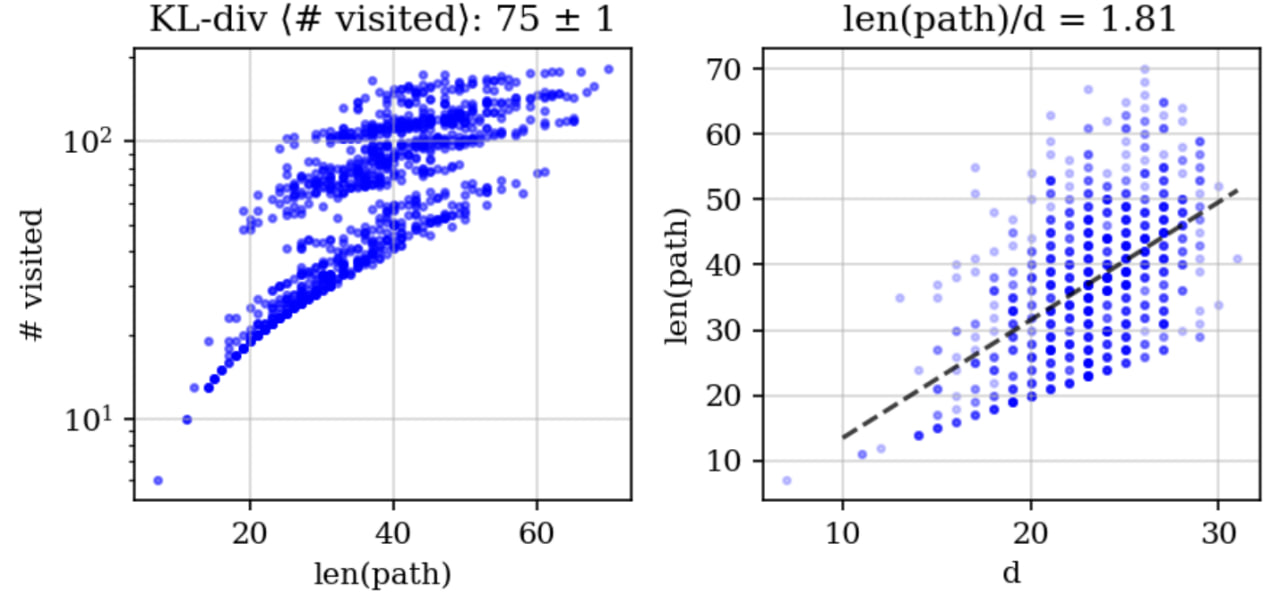
\includegraphics[width=1\textwidth]{imgs/t3.png}
	    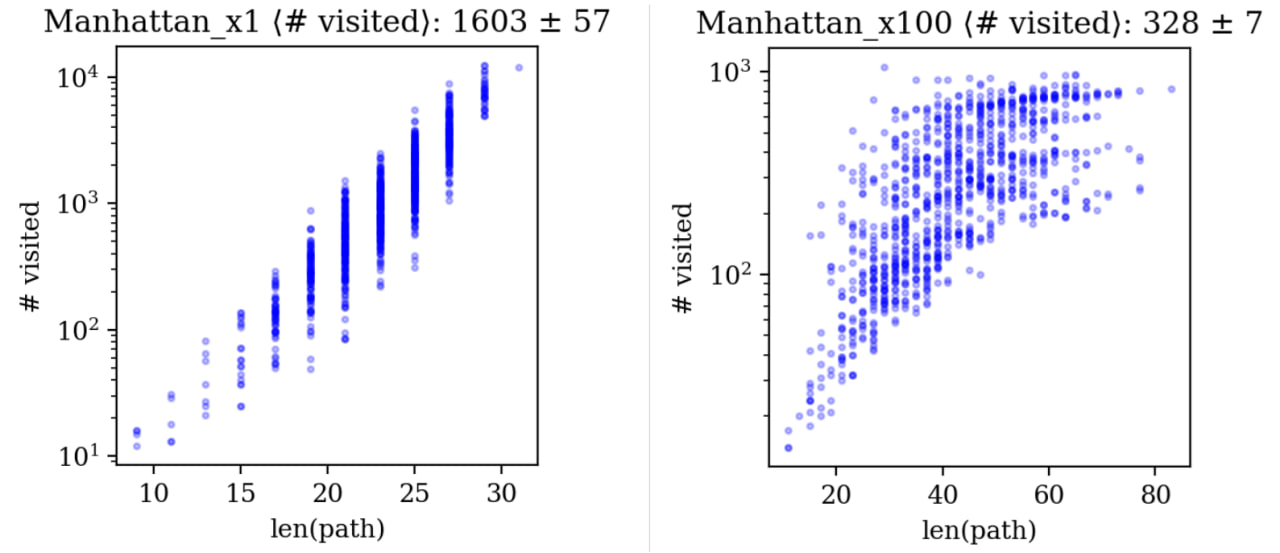
\includegraphics[width=1\textwidth]{imgs/15_1.png}
	    %\caption{}
	    %\label{fig:}
	\end{figure}
}
\end{minipage}
\hfill
\begin{minipage}{0.43\textwidth}
\onslide<2,3>{
    \begin{figure}[h]
	    \centering
	    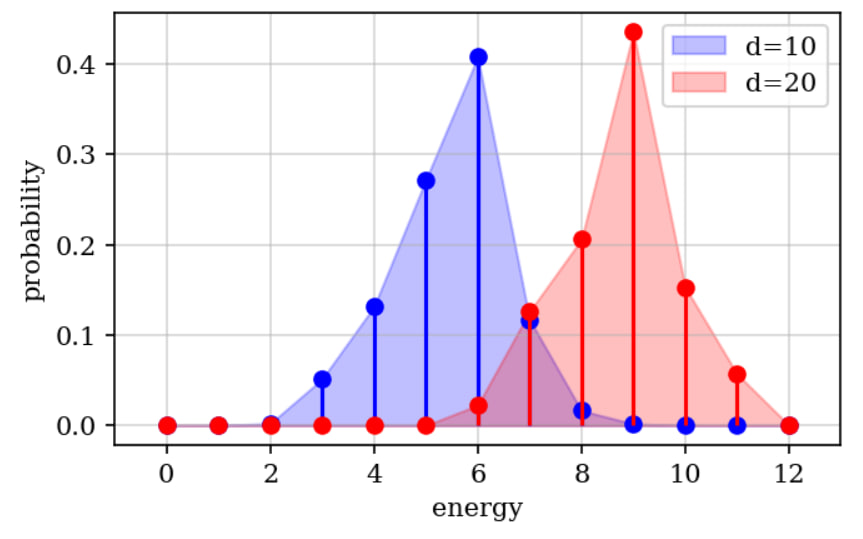
\includegraphics[width=1\textwidth]{imgs/t1.png}
	    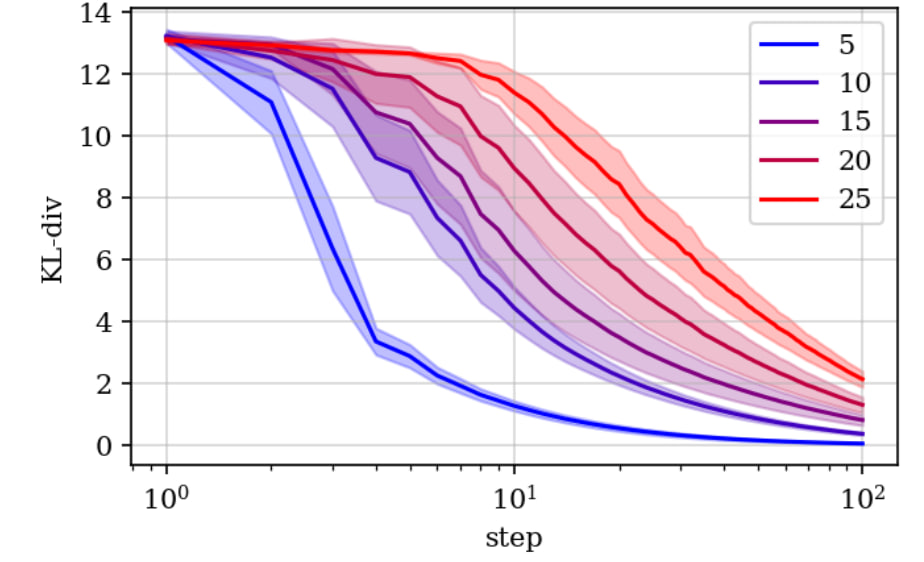
\includegraphics[width=1\textwidth]{imgs/t2.png}
	    %\caption{}
	    %\label{fig:}
	\end{figure}
}
\end{minipage}

% \phantom{42}

The behavior is highly dependent on the inverse temperature $\beta$. 

